\chapter{\label{chap:related-work}Problem description}
% Centralization of data, with the incentive of making money, naturally leads to a centralization of power. 
Music artists have a hard time making a living. The oligarchical power of music streaming services and labels squeeze the production size of the music industry. The biggest music streaming services run centralized, proprietary and closed-source software. The top 5 streaming services have 82\%, and the top 3 labels 70\% combined market share. These major corporations have huge power over both the producer and consumer sides of music streaming. Because of their power, they can ask high commission fees or lock artists to one platform. As a result, artists receive low compensation. Furthermore, the recommendation and playlist generation algorithms on streaming platforms are a black box to the user. This gives streaming and playlist companies curatorial power. A visualization of the economic muscle of both the label oligarchy and streaming platform oligarchy is shown in \ref{fig:current-music-publishing-situation}.

At the time of writing, there exists no alternative decentralized and transparent music streaming system with peer-to-peer payments directly to artists. 

\begin{figure}
    \centering
    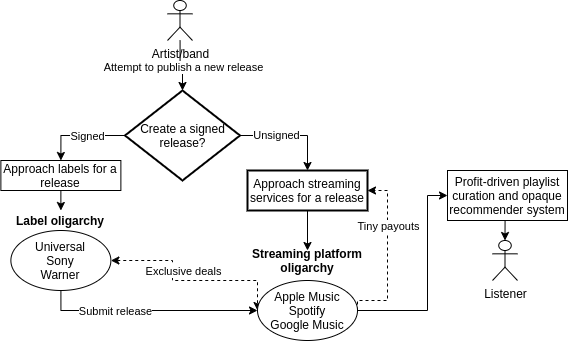
\includegraphics[width=1\linewidth]{problem-description/current-music-publishing-situation.png}
    \caption{The current flow from publishing music to receiving it as a listener. The figure shows that the framework on which music is published and found is dominated by label and streaming oligarchs and by corporate decisions.}
    \label{fig:current-music-publishing-situation}
\end{figure}

\section{History in the industry: centralization of power}
The nature of distributing music has changed spectacularly in the last 30 years. There has been a remarkable shift from physical sales, to online track downloads and piracy issues, to digital on-demand streaming. The bargaining power in music sales was once distributed over many different physical stores and labels, but is nowadays in the hand of a few labels and Big Tech corporations. According to \cite{midiamarketshare2020}, the top 5 streaming services have 82\%, and the top 3 labels 70\% combined market share (see \ref{tab:music-labels-market-share}, \ref{tab:streaming-service-market-share}). The core problem follows: ``A large number of sellers (musicians, singers, bands) are in interaction with a very small number of buyers''~\citep{rayna2009monometapoly}.

In the CD era of music, every city would have one or a few stores selling physical records. There were many music distribution companies competing for their sales. With the rapid shift towards digital sales around the 2000s, IT companies used their advantageous network infrastructures to sell digital copies to massive audiences. The downfall of the physical record stores began. At the same time, only a dozen digital stores managed to attract large audiences on their platforms, and thus survived. This marked the start of \textit{platform accumulation}~\citep{meier2019rising}: the routing of all music and money flow over centralized platforms.

Around the 2010s, the attention started to turn again to a new industry: on-demand streaming of music. This started a major transition in the last 10 years. The financial sources of the music industry changed rapidly as seen in fig. \ref{fig:music-industry-revenues}. According to \cite{friedlander2020mid}, streaming accounted for 79\% of music revenue (excluding concerts and merchandise) in the US in 2019, compared to only 15\% in 2012. Nowadays, the number of distributors to choose from is reduced to only 5 Big Tech platforms. Together they form over 80\% share of all subscribers. Clearly, streaming royalties are an increasingly important piece of income for musicians. However, these increased revenues are not felt in the pockets of musicians, but rather in major label and platform profits.

This history shows a trend towards centralization of power in the music industry. The future of artists is in the hand of a few large corporations, as they have monopoly power over them. This comes with several issues, as explained in the next section.

\begin{figure}
    \centering
    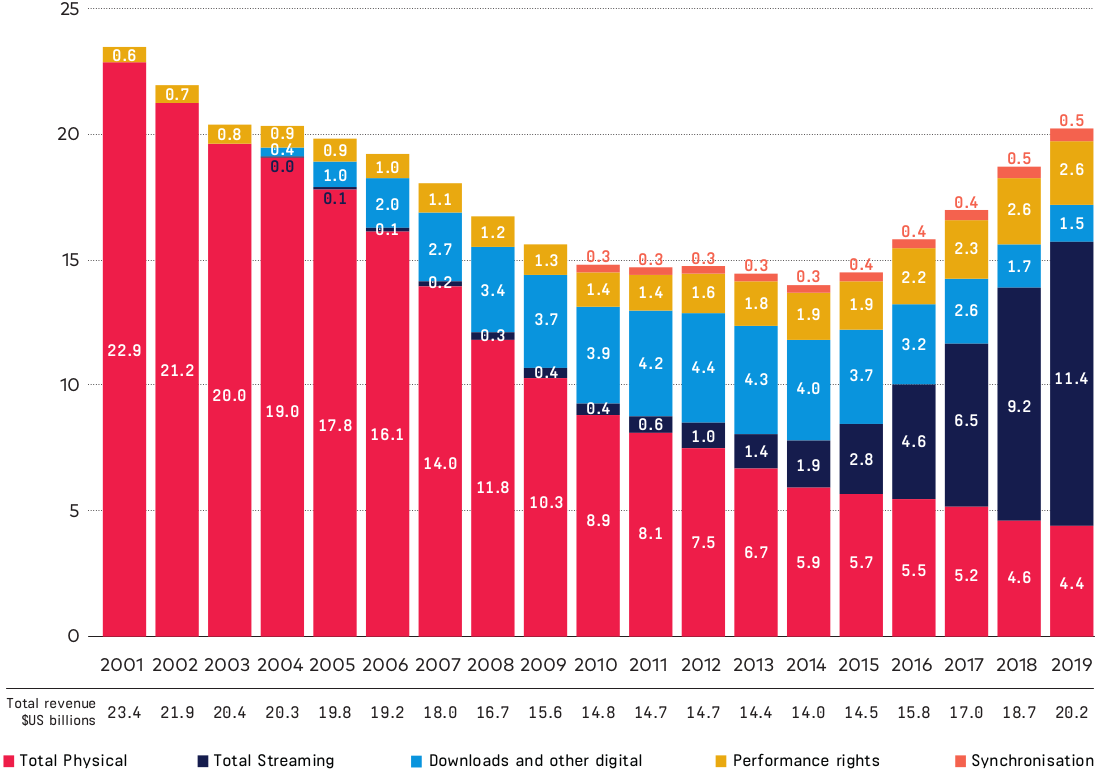
\includegraphics[width=0.75\textwidth]{problem-description/music-industry-revenues-ipfi2020.png}
    \caption{Global recorded music industry revenues (in Billion USD) (source:~\cite{ifpi2020global})}
    \label{fig:music-industry-revenues}
\end{figure}

\begin{table}[]
\centering
\begin{tabular}{|l|l|}
\hline
\textbf{Streaming service} & \textbf{Market share} \\ \hline
Spotify                    & 32\%                  \\ \hline
Apple Music                & 18\%                  \\ \hline
Amazon Music               & 14\%                  \\ \hline
Tencent Music              & 11\%                  \\ \hline
YouTube Music              & 6\%                   \\ \hline
\textbf{Total}             & \textbf{82\%}         \\ \hline
\end{tabular}
\caption{Global music streaming market share, measured by subscriber share (source:~\cite{midiamarketshare2020})}
\label{tab:streaming-service-market-share}
\end{table}

\begin{table}[]
\centering
\begin{tabular}{|l|l|}
\hline
\textbf{Major music label} & \textbf{Market share} \\ \hline
Universal Music                    & 31\%                  \\ \hline
Sony Music                & 21\%                  \\ \hline
Warner Music               & 18\%                  \\ \hline
\textbf{Total}             & \textbf{70\%}         \\ \hline
\end{tabular}
\caption{Global market share of the top 3 music labels, measured by volume of recorded music~\citep{midiamarketshare2020}}
\label{tab:music-labels-market-share}
\end{table}

\section{Monopoly power of centralized platforms}
The infrastructure of current internet applications are increasingly moving towards \textit{platformization}. In the context of music, subscriptions and purchases are majorly happening on a few central platforms, such as Spotify or Apple Music. In essence, platforms are taking control of ``the surface on which the market exchange take place'' \citep{andersson2016mastering} with digital distribution and network effects enabling an increasing centralization of power. This phenomenon is related to IT gatekeeping: tying access of content to a specific internet service. An example of this is the release of the album \textit{The Life of Pablo} in 2016, which was contracted to only be played on one platform, Tidal. 

\label{sec:problem-description-censoring}
In relation to gatekeeping, platforms are now given the task to perform moral judgments on content, for example whether to censor a certain artist. This is controversial as these judgments are no longer in the hands of democracies but rather in the hands of companies. Recent issues exist such as the disappearance of Li Zhi\footnote{\url{https://www.independent.co.uk/news/world/asia/tiananmen-square-china-li-zhi-singer-disappears-anniversary-protests-a8940641.html}}, who published songs about democracy and social issues in China. All of China's main streaming sites removed his songs. In 2019, Apple Music also removed content from their platform by singer Jacky Cheung, who referenced the tragedies of Tiananmen Square in his songs\footnote{\url{https://hongkongfp.com/2019/04/09/apple-music-china-removes-jacky-cheung-song-reference-tiananmen-massacre/}}

The latest movement in platform accumulation is the monopolization of data. Large scale of data about user interactions with the platform forms a `monopoly of knowledge' \citep{innis2007empire}. The power of platform companies are raising because platforms, in general, tend towards monopoly \citep{srnicek2017platform}. 

Aside from a monopoly, \cite{rayna2009monometapoly} interpret these platforms as \textit{monopsomies}. Monopsony power means that a dominant buyer has the power to push prices down with suppliers. In the context of music, this means that artists have little choice over which platform to publish their music on, because of the dominance of one platform. A few major players in the music industry together form an oligopolistic market. Monopsony power in this area can lead to squeezing the producer side. An example of monopsony power is an event that happened in 2014, between Amazon and Hachette. Amazon, having a large market share on e-books, used its commercial muscle to demand a larger cut of the price of Hachette books it sells. This included for all Hachette books ``preventing customers from being able to pre-order titles, reducing the discounts it offered on books and delaying shipment'' \citep{theguardian2014amazon}. 

Along the same lines, the music streaming oligarchs can use their commercial muscle to demand low pays to artists. Spotify founder and CEO Daniel Ek declared to its investors that the increase in interactions with its in-house curated playlists ``puts Spotify in control of the demand curve'' \footnote{\url{https://investors.spotify.com/financials/press-release-details/2019/Spotify-Technology-SA-Announces-Financial-Results-for-Fourth-Quarter-2018/default.aspx}}.

\section{Intermediaries take a large share}
Artists publishing their content on a music streaming service such as Google Music, Spotify and Apple Music receive low compensation, because the intermediaries take a large cut in revenue, typically between 25 and 40 percent (see \ref{tab:revenue-cuts}). The top 5 streaming services, controlling 80\% market share \citep{midiamarketshare2020}, have the power to ask high subscription fees. The Big Tech corporations behind these services are also tightly intertwined with dominant labels. For instance, \cite{aguiar2018platforms} notice that ``major record labels have substantial ownership stakes in Spotify''. \cite{meier2019rising} also point out that Big Tech platforms have shown to make lucrative deals with major labels, paying them millions of dollars up front.

According to \cite{ifpi2020global}, 2019 became the first year in which digital streaming is the single biggest source of revenue for the music industry globally. At the same time, streaming services take a large cut in revenue, and artists are having a harder time making money from music. Only a small portion of all music revenue lands in the hands of artists, as seen in fig. \ref{fig:artist-revenue}. This graph shows a large portion of revenue declared as \textit{platform costs} for streaming services, however it is unclear how much of these costs are for actual infrastructure and services and how much is for profit. According to investigations by \cite{chris2018dissecting} and \cite{recode2015}, the revenue cut of Apple Music and Spotify is between 25\% and 40\%. The largest revenue cuts are for independent musicians, which makes it very difficult to make a stable income while not contracting with the label oligarchy and music streaming oligarchy (see \ref{fig:current-music-publishing-situation}). An additional problem is opacity: streaming deals on these platforms remain behind closed doors. 

% Mention Pro-rate vs user-based model,
% Mention the recent publications from Soundcloud: "Fan Powered Royalties" https://community.soundcloud.com/fanpoweredroyalties

\begin{figure}
    \centering
    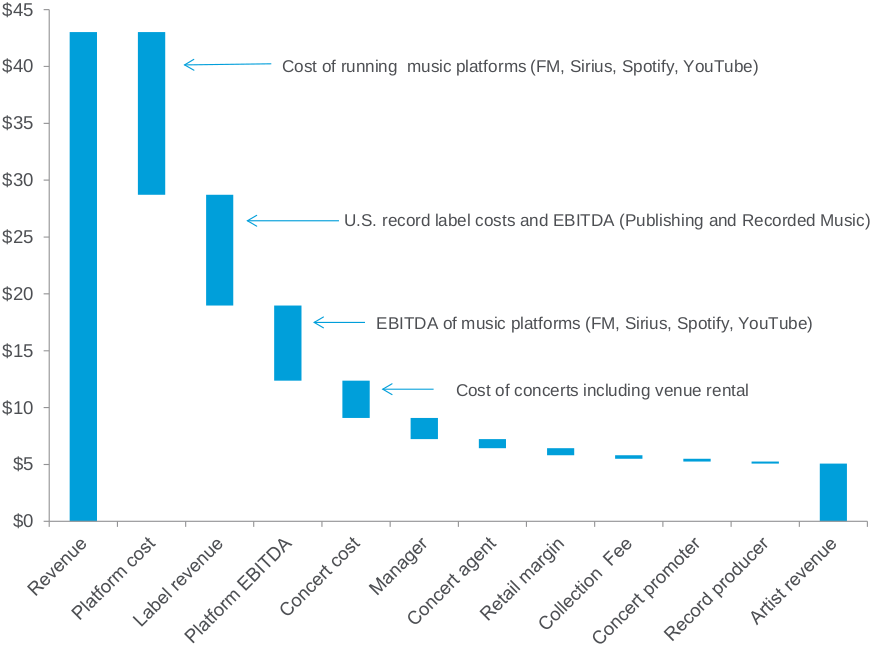
\includegraphics[width=0.65\textwidth]{problem-description/artist-revenue.png}
    \caption{Artist revenue compared to other intermediaries (source: \cite{bazinet2018putting})}
    \label{fig:artist-revenue}
\end{figure}

For these reasons, massive audiences are needed to generate sustaining profits. An investigation by Bloomberg\footnote{\url{https://www.bloomberg.com/opinion/articles/2017-09-25/the-music-business-is-more-unfair-than-ever}} shows that 152,094 Spotify subscriber streams generate only \$100 on average for artists. Consequently, only 0.733\% of all acts generate enough revenue for an artist to make a living \citep{ingham2018odds}. The International Federation of the Phonographic Industry states that as of 2018 there exists a "value gap" in digital music streaming, meaning a ``mismatch between the value that some digital platforms [...] extract from music and the revenue returned to the music community–those who are creating and investing in music'' \citep{ifpi2018global}.

\begin{table}[]
\centering
\begin{tabular}{|l|l|l|l|l|l|}
\hline
\textbf{}                      & \textbf{Music release} & \textbf{Label cut} & \textbf{Platform cut} & \textbf{Artist/band cut} & \textbf{\begin{tabular}[c]{@{}l@{}}Streams per month \\ to earn min. wage \\ (solo musician)\end{tabular}} \\ \hline
TIDAL                          & Unsigned                    & 0\%                & 40\%                  & 60\%                     & 117,760                                                                                                    \\ \hline
                               & Signed                      & 55\%               & 50\%                  & 20\%                     & 353,280                                                                                                    \\ \hline
Spotify                        & Unsigned                    & 0\%                & 40\%                  & 60\%                     & 287,574                                                                                                    \\ \hline
                               & Signed                      & 55\%               & 25\%                  & 20\%                     & 862,722                                                                                                    \\ \hline
Apple Music                    & Unsigned                    & 0\%                & 40\%                  & 60\%                     & 200,272                                                                                                    \\ \hline
                               & Signed                      & 55\%               & 25\%                  & 20\%                     & 600,816                                                                                                    \\ \hline
Google Play                    & Unsigned                    & 0\%                & 40\%                  & 60\%                     & 217,752                                                                                                    \\ \hline
                               & Signed                      & 55\%               & 25\%                  & 20\%                     & 653,256                                                                                                    \\ \hline
\textbf{This thesis challenge} & Unsigned                    & 0\%                & 0\%                   & 100\%                    & \textless 75,000                                                                                           \\ \hline
\end{tabular}
\caption{Overview of revenue cuts (estimated) on streaming platforms, with a note on the streams/plays per month that an artist should have in order to make a minimum wage. The challenge of this thesis is to liberate artists from depending on intermediaries that take a large revenue cut. Sources: \cite{thetrichordist2014}, \cite{digitalmusicnews2018}.}
\label{tab:revenue-cuts}
\end{table}

\section{Financial transparency}
\label{sec:problem-financial-transparency}
The actual overhead of the music industry is unclear, as the flow of money towards artists is either not public or lacks detail and explanation. Contract details and royalty payments are vague on purpose. This is part of the business model of music stakeholders. According to \cite{music2015fair}, ``Despite streaming services paying the same percentage of their revenue (70 percent) to rights holders as an iTunes download sale, low payouts and many intermediaries are creating concerns''~\citep{music2015fair}.

The complex flow of intermediaries results in slow and inaccurate royalty payments. As reported by \cite{bbc2019}, Eminem's publisher sued spotify because he has never been properly paid for songs that are streamed on Spotify for billions of times. The court mentioned that the streaming service ``[...] lacked the infrastructure needed to make sure songs are licensed and musicians are paid''. Royalty payments are generally also unnecessarily time-consuming: it can take 6 to 12 months to arrive at artists~\citep{music2015fair}. 

It appears that a large amount of royalty revenue flows outside of the artists, in a ``black box''~\citep{music2015fair}. The reason is that there is no industry-wide system for declaring rightful owners of music. This problem is even more significant as there is no incentive for the major labels and major streaming services to improve this situation. These companies deliberately obfuscate royalty processing, or use outdated and unnecessarily complex systems.

\section{Profit-driven recommendation engines}
\label{sec:problem-description-recommendations}
The Big Tech music companies recommend content that best fits their business model, which may be contrary to what is most useful to their customer. The companies can promote or dis-promote content by their choosing. This shows ``curatorial power'': the ability to advance own interests by organizing and prioritizing content \citep{prey2020locating}.

Musicians and record labels are increasingly dependent on landing on Spotify-curated playlists. For example, a study done by the European Commission shows that, for a track to land on the Spotify-curated playlist `Today's Top Hits', it will see an increase of \$163,000 in revenue \citep{aguiar2018platforms}. 99 of the top 100 playlists are curated by the streaming company. So its recommendation algorithms and playlist curation systems are highly influential. 

A major problem with this situation is that the inner workings of the recommendation algorithms are opaque to the user. These algorithms, fed by user interaction data, are in some extend also a black box to the company, as they are built using machine learning technologies. However, as noted by \cite{gillespie2014relevance}, the impression that algorithms are objective is a ``carefully crafted fiction''. Namely, they are altered based on company strategies. \cite{thebaffler2017} describes that ``[the Spotify front page] is tightly controlled by Spotify’s staff and dictated by the interests of major labels, brands, and other cash-rich businesses who have gamed the system''.

Companies are not obliged to explain their algorithms. In the context of recommendations, this leads to a ``threat of invisibility": the problem of content regularly disappearing \citep{bucher2018if}, a phenomenon which is out of the hands of the artist, because the artist lacks knowledge in the algorithm workings. Frustrating for artists and labels is also the vagueness of getting playlisted: it is unclear why ``[...] a particular track was placed, or replaced, on a playlist'' \citep{prey2020locating}. 

On the other hand, if the playlist curation is performed by a person or company, we run into another issue. This is depicted in a recent book by \cite{heuvelings2020}. The author had the job of maintaining several high-demand playlists on Spotify, with millions of monthly listeners. This gave her substantial power but also huge (financial) pressure from artists and labels, demanding their work to be visible on her playlists. This makes the music industry even more unfair for smaller artists with less power.

\section{Research question}
All in all, the main issue is as follows. The music industry is imbalanced: it suffers from centralized power that is in the hand of a few labels and Big Tech corporations. Our research question thus follows:

\textit{How can we design and implement a music streaming service that distributes the power from one authority to its users?}
% \subsection{Copyright orthodoxy} ?
% % https://search.proquest.com/openview/2ea25b1bed66750c91cdbc6ea2a5093a/1